\chapter{Introduction}
\vspace*{0.5cm}
\setcounter{page}{1}
\pagenumbering{arabic}

Since the start of 2020 \textit{Sars-COVID19} has initiated a world-wide pandemic. In an attempt to slow down the fast and uncontrollable spreading of this disease various prevention and diagnosis methods have been developed. In this work, out of all these various methods, the attention is going to be put on diagnostic methods related to medical images, be they automatic or semi-automatic, to be intended either as Clinical Decision Support Systems (CDSS) or as a quick evaluation to completely avoid human analysis.
In this light this first introductory chapter is going to start from a basic theoretical overview of the necessary core concepts that will be needed throughout this whole work such as definition of an image and imaging methods, with particular attention to medical methods. This will be followed by an introduction to Artificial Intelligence (AI) and some Machine Learning techniques. Finally some of the concepts from the two previous topics will be treated jointly under the discipline of radiomics, which will be defined and explored as necessary.

\section{Theoretical background: Medical Images}
In this section the objective is to simply provide a set of basic definitions pertaining to images as well as a general introduction to the methods used to create said images. Firstly images are a means of representing in a visual way a physical object or set thereof, when talking about images it's common to refer specifically to digital images.

\begin{definition}[Digital Image]
A numerical representation of an object; more specifically an ordered array of values representing the amount of radiation emitted (or reflected) by the object itself. The values of the array are associated to the intensity of the radiation coming from the physical object; to represent the image these values need to be associated to a scale and then placed on a discrete 2D grid. 
To store these intensities the physical image is divided into regular rectangular spacings, each of which is called pixel\footnote{The term pixel seems to originate from a shortening of the expression Picture's (pics=pix) Element(el). The same hold for voxel which stands for Volume Element}, to form a 2D grid; inside every spacing is then stored a number (or set thereof) which measures the intensity of light, or color, coming from the physical space corresponding to that grid-spacing. 
The term digital refers to the discretization process that inherently happens in storage of the values, called pixel values, as well as in arranging them within the grid. It's possible to generalize from 2D images to 3D volumes, simply by stacking images of the same object obtained at different depths. In this context, the term pixel is substituted by voxel, however since they are used interchangeably in literature they will, from now on, be considered equivalent.
\end{definition}

Generally pixel values stored as integers p$\in$ [0,2$^{n}$-1] with p,n$\in$ $\mathbb{N}$  or as p$\in$[0,1] with p$\in$ $\mathbb{R}$, the type of value stored within each pixel changes the nature of the image itself. 
A single value is to be intended as the overall intensity of light coming from the object and is used for a gray-scale representation, a set of three\footnote{The three values correspond each to the intensity of a single color, the most commonly used set of colors is the RGB-scale (Red, Green, Blue). Further information can be found by looking into Tristimulus theory\cite{Tristimulus}}  or four\footnote{Same as RGB but with four colors, the most common scale is CMYK (Cyan, Magenta, Yellow, blacK)} values can be intended as a color image.

\begin{figure}[H]
     \centering
     \subfloat[][\centering RGB color space on a cube]{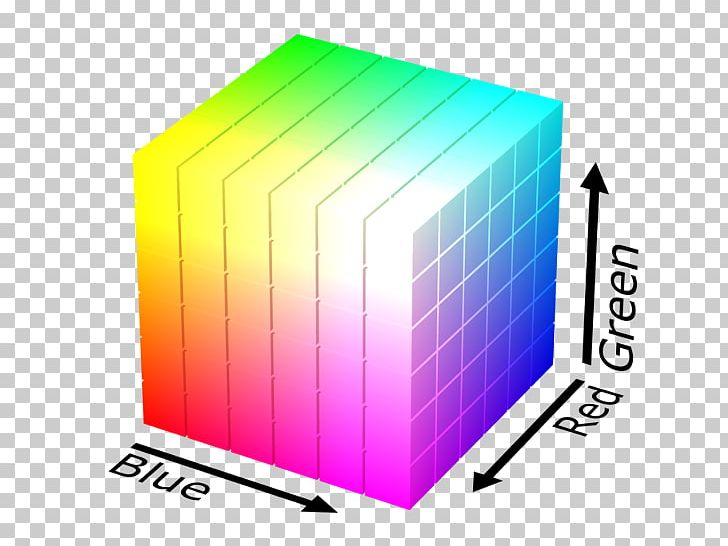
\includegraphics[width=5cm]{RGB_cube.jpg}\label{fig: RGB_cube}}
    \qquad
     \subfloat[][\centering HSV cone]{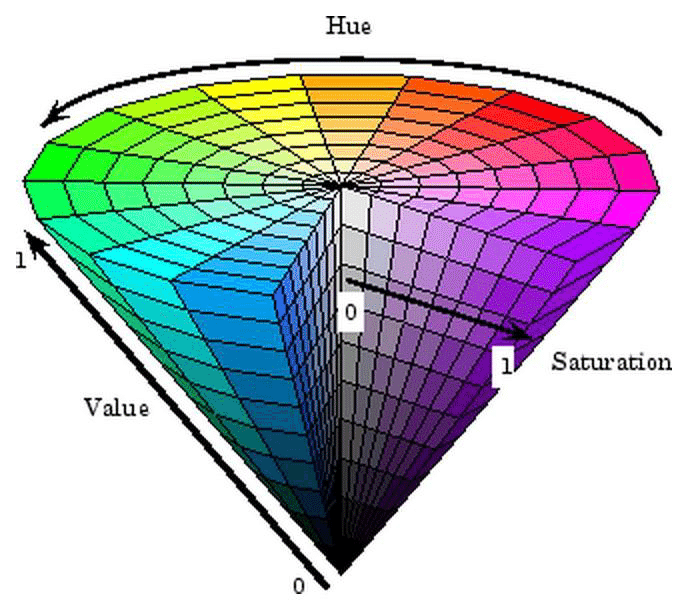
\includegraphics[width=5cm]{HSV_cone.png}\label{fig:HSV_cone}}
     \caption{Examples of color spaces}
     \label{fig:color_spaces}
\end{figure}

There are a lot of possible scales for representation\footnote{Besides RGB and CMYK \ref{fig: RGB_cube} the most common color spaces are CIE (Commision Internationale d’Eclairage) and HSV fig:\ref{fig:HSV_cone} (Hue,Saturation and Value). Refer to \cite{Color_spaces} for further details}, which are sometimes called color-spaces, however the most noteworthy in the scope of this work is the Hounsfield unit (HU) scale.

\begin{definition}[Hounsfield unit (HU)]
A scale used specifically to describe radiodensity, frequently used in the context of CT (Computed Tomography) exams. The values are obtained as a transformation of the linear attenuation coefficient of the material being imaged and, since the scale is supposed to be used on humans, it's defined such that water has value zero and air has the most negative value -1000. For  a more in depth discussion refer to \cite{Hounsfield}
\end{definition}

\begin{equation}\label{eq:HU_def}
    HU = 1000*\frac{\mu - \mu_{H_2O}}{\mu_{H_2O} - \mu_{Air}}
\end{equation}

The utility of this scale is in it's definition, since the pixel value depends on the attenuation coefficient it's possible to individuate a set of ranges that identify, within good reason, the various  tissues in the human body: for example lungs are [-700, -600] while bone can be in the [500, 1900] range.
A more in depth discussion of the topics relative to Hounsfield units is going to be carried out at a later point throughout this chapter, in the meantime it's necessary to clarify what are the most important characteristics of an image:

\begin{itemize}
\item Spatial Resolution: A measure of how many pixel are in the image or, equivalently, how small each pixel is; a larger resolution implies that smaller details can be seen better fig:\ref{fig:resolution_types}. Can be measured as the number of pixel measured over a distance of an inch ppi(Pixel Per Inch) or as number of line pairs that can be distinguished in a mm of image lp/mm (line pair per millimeter).
\item Gray-level Resolution: The range of the pixel values, a classic example is an 8-bit resolution which yields 256 levels of gray. A better resolution allows a better distinction of colors within the image fig:\ref{fig:resolution_types}.

\begin{figure}[H]
  		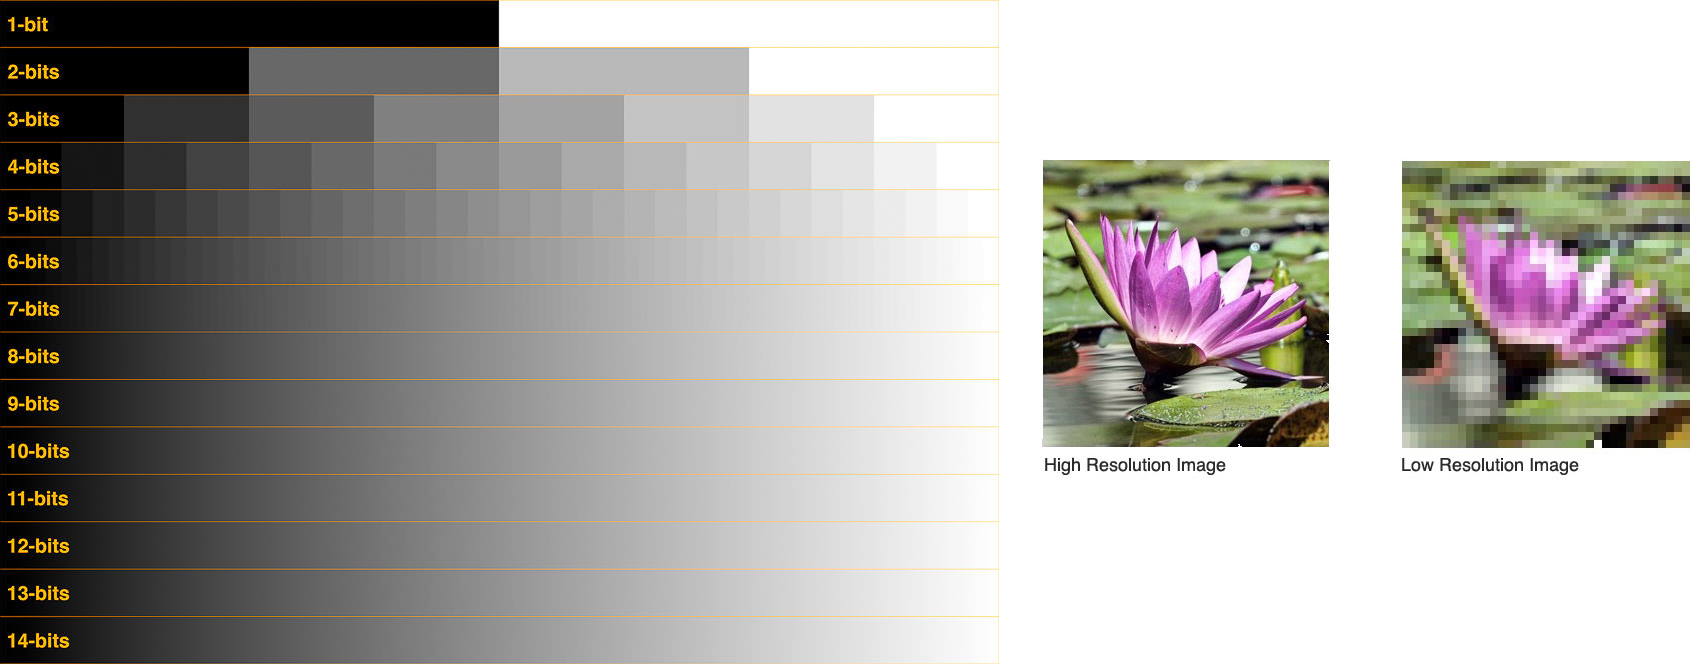
\includegraphics[width=0.8\textwidth]{Img_resolution.png}
        \caption{Example of visual differences in Gray-level (left) and spatial (right) resolution \label{fig:resolution_types}}
\end{figure}

\item Size: Refers to the number of pixel per side of the image, for example in CT-derived images the coronal slices are usually 512x512. These numbers depend on the acquisition process and instrument but in all cases these refer to the number of rows and columns in the sampling grid as well as in the matrix representing the image.
\item Data-Format: How the pixel values are stored in the file of the image. The most commonly used formats are .PNG and .JPG however there are a lot of other formats. In the context of this work, which is going to be centered on medical images, the most interesting formats are going to be the nii.gz (Nifti) and the .dcm (DICOM). The first contains only the pixel value information hence it's a lighter format, it originates in the field of Neuroimaging\footnote{In fact Nifti stands for Neuroimaging Informatics Technology Initiative (NIfTI)}, it is used mainly in Magnetic resonance images of the brain but also for CT scans and, since it contains only  numeric information, it's the less memory consuming option out of the two. The second contains not only the image data but also some data on the patient, such as name and age, and details on how the exam was carried out, such as machine used and specifics of the acquisition routine. This format is heavier than the previous one and, for privacy purposes, is much more delicate to handle which is why it's anonymization of the data needs to be taken in consideration. For a thorough description of the DICOM standard refer to \cite{DICOM}. 
\end{itemize}

The format in which the image is saved depends on the compression algorithm used to store the information within the file. These algorithms can be lossy, in which case some of the information is lost to reduce the memory needed for storage, or lossless which means that all the information is kept at the expense of memory space. The first set of methods is preferred for storage of natural images, these are cases in which details have no importance, whereas the second set of methods is used where minute details can make a considerable difference such as in the medical field\footnote{A detailed description of compression algorithms is beyond the scopes of this thesis, for this reason please refer to \cite{Img_Compression} for more information}.
Given this set of characteristics it should now be clear that images can be thought of as array of numbers, for this reason they are often treated as matrices and, as such, there is a well defined set of valid operations and transformations that can be performed on them. All these operations and transformations, in a digital context\footnote{As opposed to analog context, which would mean the chemical processes used at the start of photography to develop and modify the film on which the image was stored}, are performed via computer algorithms which allow almost perfect repeatability and massive range of possible operations. 
Given the list-like nature of images one of the most natural things to do with the pixel values is to build an histogram to evaluate some of the characteristic values of their distribution, such as average, min/max, skewness, entropy... . The histogram of the image, albeit not being an unambiguous way to describe images, is very informative. When looking at an histogram it's immediately evident whether the image is well exposed and if the whole range of values available is being used optimally. 

\begin{figure}[H]
  		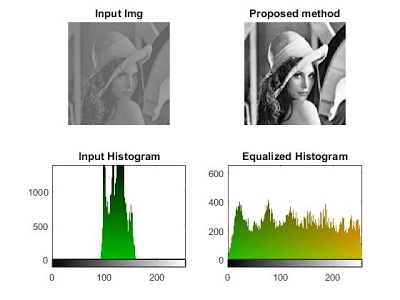
\includegraphics[width=0.8\textwidth]{Contrast_enhancement.jpg}
        \caption{Example of differences in contrast due to histogram equalization\label{fig:contrast_enhancement}}
\end{figure}

This leads us to the concept of \textit{Contrast} which is a quantification of how well different intensities can be distinguished. If all the pixel values are bundled in a small range leaving most of the histogram empty then it's difficult to pick up the differences because they are small however, if the histogram has no preferentially populated ranges then the differences in values are being showed in the best possible way fig:$\ref{fig:contrast_enhancement}$. Note also that if looking at the histogram there are two(or more) well separated distributions it's possible that these also identify different objects in the image, which will for example allow for some basic background-foreground distinction.
Assuming they are being meaningfully used \footnote{For example adding/subtracting one image to/from another can be reasonably understood, multiplying/dividing are less obvious but still used e.g. in scaling/mask imposition and change detection respectively} all mathematical operations doable on matrices can be performed on images for this reason it would be useless to list them all. However, it's useful to provide a list of categories in which transformations can be subdivided:

\begin{enumerate}
\item Geometric Transformations involve the following steps:
		\begin{enumerate}
		\item Affine transformations: Transformations that can can be performed via matrix multiplication such as rotations, scaling, reflections and translations. This step basically involves computing where each original pixel will fall in the transformed image
		\item Interpolation: Since the coordinates of the transformed pixel might not fall exactly on the grid it might become necessary to compute a kind of average contribution of the pixel around the destination coordinate to find a most believable value. Examples of such methods are linear, nearest neighbour and bicubic. 
		\end{enumerate}
\item Gray-level (GL) Transformations: Involve operating on the value stored within the pixel, these can be further subdivided as:
		\begin{enumerate}
		\item Point-wise: The output value at specific coordinates depends only on the output value at those same specific coordinates. Some examples are window-level operations, thresholding, negatives and non-linear operations such as gamma correction which is used in display correction. Taken p as input pixel value and q as output and given a number $\gamma \in \mathbb{R}$, gamma corrections are defined as:
		\begin{equation}
		q = p^{\gamma}
		\end{equation}
		\item Local: The output value at specific coordinates depends on a combination of the original values in a neighbourhood around that same coordinates. Some examples are all filtering operation such as edge enhancement, dilation and erosion. These filtering methods are based on performing convolutions which will be explained in \ref{sec:Convolution}
		\item Global: The output value at specific coordinates depends on all the values of the original images. Most notable operation in this category is the Discrete Fourier Transform and it's inverse which allow switching between spatial and frequency domains. It's worth noting that high frequency encode patterns that change on small scales whereas low frequencies encode regions of the image that are constant or slowly varying.
		\end{enumerate}
\end{enumerate}

The aforementioned is surely not a comprehensive list of all that can be said on images however it should be enough for the scopes of this work, having seen what constitutes and image and what can be done with one it becomes interesting to explore how images are obtained. The following discussion is going to introduce briefly some of the methods used to obtain medical images, getting more in depth only on the modality used to obtain all the images used in this thesis which is Computed Tomography.

\begin{enumerate}
\item Magnetic Resonance Imaging (MRI): This technique is based on the phenomenon of Nuclear Magnetic Resonance(NMR) which is what happens when diamagnetic atoms are placed inside a very strong uniform magnetic field are subject to Radio Frequency (RF) stimulus. These atoms absorb and re-emit the RF and supposing this behaviour can somehow be encoded with a positional dependence then it's possible to locate the resonant atoms given the response frequency measured. Suffices to say that this encoding is possible however the setup is very complex and the possible images obtainable with this method are very different and can emphasize very different tissue/material properties. Nothing more will be said on the topic since no data obtained with this methodology will be used. More details can be found in \cite{MRI}
\item Ultra-Sound (US): The images are obtained by sending waves of frequency higher to those audible by humans and recording how they reflect back. This technique is used mainly in imaging soft peripheral tissues and the contrast between tissues is given by their different responses to sound and how they generate echo. The main advantages such as low cost, portability and harmlessness come at the expense of explorable depth, viewable tissues, need for a skilled professional and dependence on patient bodily composition as well as cooperation.
\item Positron Emission Tomography (PET): In this case the images are obtained thanks to the phenomenon of annihilation of particle-antiparticle, specifically of positron electron.	The positrons come from the $\beta ^+$ decay of a radio-nucleide bound to a macromolecule, which is preferentially absorbed by the site of interest \footnote{Most commonly Fluoro-DeoxyGlucose FDG which is a glucose molecule labelled with a $^{18}$F atom responsible of the $\beta ^+$ decay. In general these radio-pharmaceuticals are obtained with particle accelerators near, or inside, the hospital that uses them. They are characterized by the activity measured as decay/s $\doteqdot$ Bq (read Becquerel) and half-life $\doteqdot$ T$_{\frac{1}{2}}$ which is how long it takes for half of the active atoms to decay}. Once the annihilation happens a pair of (almost) co-linear photons having (almost) the same energy of 511 keV is emitted, the detection of this pair is what allows the reconstruction of the image representing the pharmaceutical distribution within the body. Once again there are a lot of subtleties that are beyond the scopes of this thesis, suffices to say that: firstly the exam is primarily used in oncology given the greater energy consumption, hence nutrients absorption, of cancerous tissue and secondly this technique can be combined with CT scans to obtain a more detailed representation of the internal environment of the patient
\end{enumerate}

The last technique that is going to be mentioned is Computed Tomography however, given it's relevance inside this thesis work, it seems appropriate to describe it in a dedicated section.

\subsection{X-ray and Computed Tomography (CT)}
Let's start by considering the word Tomography, it comes from the greek $\textit{Tomo}$ which means "to cut". This technique originates as an advancement of planar x-ray imaging, which follows the same physical principles yet has some major limitations main of which being the lack of depth information. Since x-ray planar imaging involves seeing how a beam of x-rays changes after traversing a target, the process amounts to a kind of average of all the effects occurred over the whole depth travelled. 
The step-up in performance is due to the possibility of building 3D images by imaging different slices of the patient and digitally recording them as data on a computer. This process of storing slices gives the name Computed Tomography\footnote{From the greek word for "to cut" \textit{tomo}}. 
In both cases the description of the data acquisition process can be summarized as follows: First x-rays are somehow generated by the machine, these x-rays are then focused and positioned such that they mostly hit the region that needs imaging. Once the beam starts interacting with the imaged object\footnote{In this case it's always going to be a patient, however this process is general and is also used in industry to investigate object construction} it gets attenuated according to the material it's made of. Having then travelled across the whole object it interacts with a sensor, be it film, semiconductor or other, which stores some data that will then reconstructed to constitute the final image. This final step is performed following a (tomographic) reconstruction algorithm which given a set of 2D projections returns a single 3D image.
In this light the interesting processes are how the radiation is created and shaped before hitting the patient and how said radiation then interacts with the matter of both the patient's body and the sensor beyond it. 


\subsubsection{Generation and management of radiation: The CT scanner}

\subsubsection{Radiation-matter interaction: Attenuation in body and measurement}



\section{Theoretical background: Artificial Intelligence (AI)}

\subsection{Convolution}\label{sec:Convolution}

\section{Combining radiological images  with AI: Radiomics}



\begin{equation}\label{eq:1}
    EM=\int n_e^2~dl\approx\left \langle n_e \right \rangle^2l\qquad \mathrm{pc ~cm^{-6}},
\end{equation}

\vspace*{0.8cm}
\begin{table}[H]
    \centering
    \caption{esempio di tabella e label associati \label{tab:param}}
    \label{parametri}
    \begin{tabular}{@{}lllll@{}}
    \toprule
    Class of Region & \begin{tabular}[c]{@{}l@{}}Size\\ (pc)\end{tabular} & \begin{tabular}[c]{@{}l@{}}Density\\ ($\mathrm{cm^{-3}}$)\end{tabular} & \begin{tabular}[c]{@{}l@{}}$EM$\\ ($\mathrm{pc\:cm^{-6}}$)\end{tabular} & \begin{tabular}[c]{@{}l@{}}Ionized Mass\\ ($\mathrm{M_\odot}$)\end{tabular} \\ \midrule
    Hypercompact & $0.03$ & $10^6$ & $10^{10}$ & $10^{-3}$ \\
    Ultracompact & $0.1$ & $10^4$ & $10^7$ & $10^{-2}$ \\
    Compact & $0.5$ & $5\cdot 10^3$ & $10^7$ & $1$ \\
    Classical & $10$ & $100$ & $10^2$ & $10^5$ \\
    Giant & $100$ & $30$ & $5\cdot 10^5$ & $10^3-10^6$ \\
    Supergiant & $100$ & $10$ & $10^5$ & $10^6-10^8$ \\ 
    \bottomrule
    \end{tabular}
\end{table}




\newpage
\section{Digital Images}

\begin{figure}[H]
        \vspace*{1cm}
  		\makebox[\textwidth][c]{\includegraphics[width=\textwidth]{W3M.eps}}
        \caption{esempio di figura con label associata \label{fig:W3M}}
\end{figure}

\subsection{Medical Imaging methodologies}

\section{Artificial Intelligence}
\section{AI in medicine: feature extraction and segmentation}